% !TeX root = ../libro.tex
% !TeX encoding = utf8

\chapter{Introducción}  \label{ch:Introduccion_informatica}

\noindent En los últimos años, el desarrollo de la Inteligencia Artificial \cite{norvig2002modern} ha permitido que tareas que antes se consideraban lentas o complicadas se puedan llevar a cabo con mayor rapidez y precisión. En cambio, hay otras que, incluso para expertos en la materia, todavía resultan complicadas de resolver de forma rápida y precisa. El presente trabajo de fin de grado (TFG) se ocupa de una de estas tareas: la localización automática de landmarks cefalométricos en fotografías para tareas de identificación humana forense. 

\medskip

\noindent Nos encontramos pues en el ámbito de las \textbf{ciencias forenses}. Aquellas que aplican el método científico a hechos presuntamente delictivos, con la finalidad de aportar pruebas a efectos judiciales. Dentro de este campo destacan principalmente dos disciplinas: 

\begin{itemize}
    \item La \textbf{Criminalística}: disciplina encargada del descubrimiento y verificación científica de presuntos hechos delictivos y quienes los cometen.
    \item La \textbf{Medicina Forense}: disciplina encargada de determinar el origen de las lesiones, las caisas de muerte o la identificación de seres humanos vivos o muertos.
\end{itemize}

\medskip

\noindent Dentro de la medicina forense se encuentra la \textbf{antropología forense}, que principalmente se encarga de la identificación de personas a partir de restos óseos. Y es en este ámbito donde se encuentran los procesos que dan sentido a este trabajo. 


\section{Descripción del problema y Motivación}

    \noindent Los \textbf{landmarks cefalométricos} son puntos localizados en la cara que nos permiten caracterizar la morfología de la cabeza. La correcta identificación de estos puntos es de extrema importancia en tareas como la extracción de índices de proporción antropométricos (por ejemplo, para problemas de clasificación o detección de patologías), la comparación facial forense y la identificación humana forense mediante la superposición craneofacial (SCF), en el cual se comparan imágenes de la persona difunta (imágenes ante-mortem) con una representación 3D de un cráneo candidato, con el fin de determinar si el cráneo pertenece a la persona de las imágenes o no. La correspondencia entre cara y cráneo se hace con ayuda del marcado en el cráneo de landmarks \textit{craneométricos}. Así, cada landmark \textit{cefalométricos} tiene un homólogo \textit{craneométrico} con el mismo nombre. En la \autoref{fig:procesoSCF}  podemos ver un esquema del proceso seguido.

    \medskip

    \noindent El marcado de landmarks cefalométricos no es una tarea sencilla, pues depende de factores diversos a tener en cuenta como son la calidad de la imagen, la posición del sujeto o el tejido blando facial (que separa el punto craneométrico de su homólogo cefalométrico). El desplazamiento ocasionado por el tejido blando facial no es constante ni se produce siempre en la misma dirección, podemos ver un ejemplo de este hecho en la \autoref{fig:landmarks_marcados}. Estos problemas, ocasionan que el experto forense tarde mucho en la tarea del marcado de landmarks y que el proceso sea difícilmente replicable. Por esto, pese a los avances actuales que se están llevando a cabo para automatizar esta tarea \cite{Huete2015PastPA}, la identificación de landmarks cefalométricos sigue realizándose a mano normalmente. En este contexto, el presente trabajo tratará de proporcionar una solución automática al proceso del marcado de \textbf{landmarks cefalométricos}.
    \begin{figure}[H]
        \centering
        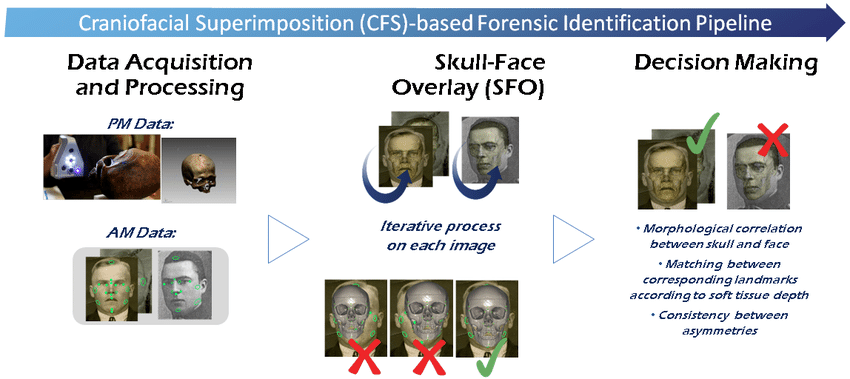
\includegraphics[width=0.95\textwidth]{img/SCF.png}
        \caption{Etapas del proceso de superposición craneofacial. En primer lugar se realiza la recogida de imágenes ante-mortem (AM) y muestras post-mortem (PM) junto con el marcado de landmarks y escaneo $3D$ del cráneo candidato. Tras esto comienza el experto comienza el proceso iterativo en el que trata de hacer coincidir los landmarks cefalométricos y craneométricos. Finalmente se realiza una toma de decisiones en función de los resultados obtenidos. Imagen extraída de \cite{article}.}
        \label{fig:procesoSCF}
    \end{figure}
    \begin{figure}[H]
        \centering
        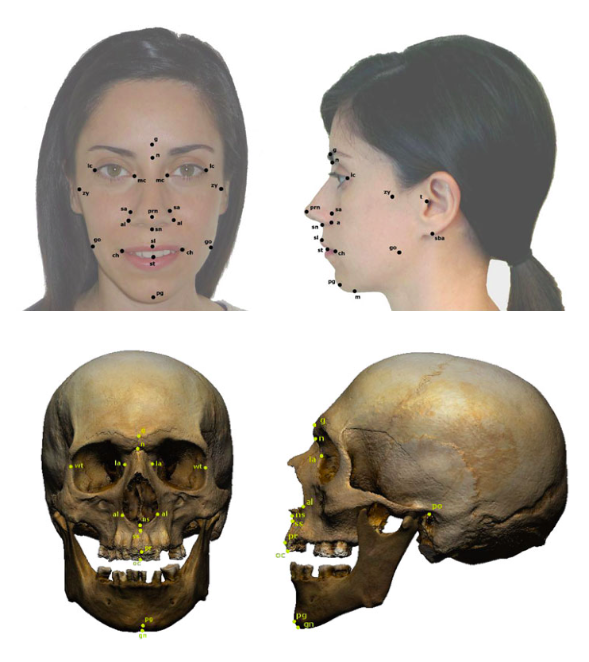
\includegraphics[width=0.7\textwidth]{img/marcado_landmarks.png}
        \caption{En esta imagen podemos ver la correspondencia entre landmarks craneométricos y cefalométricos. Algunos de los landmarks que aparecen en la imagen serán estudiados en este trabajo. Imagen extraída de \cite{damas2020handbook}.}
        \label{fig:landmarks_marcados}
    \end{figure}

    \medskip 

    \noindent Por otro lado, el reconocimiento de \textbf{landmarks faciales} (puntos de referencia marcados en la cara sin justificación biológica) es una tarea muy investigada actualmente, de la que existen  multitud de trabajos resueltos en su mayoría usando algoritmos de \textbf{deep learning}. Pese a no guardar relación con la morfología del cráneo, este tipo de landmarks son de gran utilidad para la identificación de personas en vídeos, el reconocimiento de gestos y posición de la cara o determinar la dirección en la que un individuo mira. 

    \medskip

    \noindent Para entrenar dichos algoritmos, se cuenta con multitud de bases de datos y ejemplos etiquetados, a diferencia que con los landmarks cefalométricos. Así, en este trabajo vamos a tratar de tomar una CNN experta en el reconocimiento de landmarks faciales en imágenes \textit{in-the-wild} (conjunto de imágenes tomadas en situaciones no controladas de iluminación, pose o calidad), y vamos a tratar de especializarla en el marcado de \textbf{landmarks cefalométricos} aprovechando el conocimiento que ya poseen. En particular nos hemos fijado en el framework \textbf{3FabRec}\cite{browatzki20203fabrec}. Dicho framework cuenta con excelentes resultados en la tarea de detección de landmarks en imágenes y sobre todo nos interesa porque obtiene buenos resultados entrenando con pocas imágenes, algo que nos puede ser de utilidad teniendo en cuenta los pocos datos de los que se disponen. Así, se pretende diseñar un modelo capaz de aprender a marcar un total de $30$ landmarks, que podemos ver en la \autoref{table:tabla_landmarks}. 

    \begin{table}
        \centering
        \caption{Landmarks que se intentarán predecir.}
        \begin{tabular}{ |c|l|l|c| } 
            \hline
            & \textbf{Landmarks} & \textbf{Notación} \\
            \hline
            1 & Menton & Me \\ 
            2 & Gnathion & Gn \\ 
            3 & Pogonion & Pg \\ 
            4 & Prosthion & Pr \\ 
            5 & Labiale Superius & Ls \\ 
            6 & Subnasale & Sn \\ 
            7 & Nasion & N \\ 
            8 & Glabella & G’ \\ 
            9 & Vertex & v \\ 
            10 & Left Gonion & GoL \\ 
            11 & Right Gonion & GoR\\ 
            12 & Left Zygion & zyL \\ 
            13 & Right Zygion & zyR\\ 
            14 & Left Alare & alL \\ 
            15 & Right Alare & alR \\ 
            16 & Left Endocanthion & EnL \\ 
            17 & Right Endocanthion & EnR \\ 
            18 & Left Exocanthion & ExL \\ 
            19 & Right Exocanthion & ExR \\ 
            20 & Left Tragion & T’L \\ 
            21 & Right Tragion & T’R \\ 
            22 & Infradentale & Id \\ 
            23 & Trichion & Tr \\ 
            24 & Supramentale & sm\\ 
            25 & Left Frontotemporale & FtL \\ 
            26 & Right Frontotemporale & FtR \\ 
            27 & Left Frontozygomaticus & fzL \\ 
            28 & Right Frontozygomaticus & fxR \\ 
            29 & Left Midsurpaorbital & msoL \\ 
            30 & Right Midsupraorbital & msoR \\ 
            \hline
        \end{tabular}
        \label{table:tabla_landmarks}
    \end{table}


    \medskip

    \noindent En este contexto, el presente TFG comparte el mismo problema que el TFG realizado por Guillermo Gómez en $2019$, que representa una medida del estado del arte en este campo, por lo que compararemos los resultados obtenidos por su modelo con los que obtengamos en este trabajo. Además, el enfoque de los datos a usar es distinto, pues aunque partimos del mismo dataset, vamos a explorar técnicas de \textit{few-shot learning}, es decir, trataremos de obtener un modelo competente con pocos datos de entrenamiento. Mientras que en este trabajo se amplió el conjunto de entrenamiento con un dataset extra de modelos $3D$ de rostros con landmarks anotados de los que se extrajeron proyecciones $2D$.



    \subsection{Base de datos proporcionada}
        \noindent El conjunto de datos Forense que se proporciona para resolver el problema presenta las siguientes características: 

        \begin{itemize}
            \item Contienen un total de \textbf{167 imágenes} de distintos sujetos \textit{in-the-wild}. El número de imágenes por sujeto no se distribuye de forma equitativa, algunos solo disponen de una imagen mientras que otros tienen varias. El sujeto con mayor número de imágenes tiene siete.
            \item La resolución de las imágenes también varía mucho, oscilando entre los $4350 \times 3400$ píxeles y $168 \times 256$ píxeles.
            \item Hay imágenes a color y en escla de grises.
            \item Las imágenes se presentan en un conjunto muy variado de posiciones. Disponemos de: 
            \begin{itemize}
                \item $87$ imágenes frontales.
                \item $57$ imágenes con rostros en posición de \textbf{$3/4$}.
                \item $23$ imágenes de perfil.
            \end{itemize}
            \item Hay hasta un total de $30$ landmarks que pueden marcarse. Sin embargo, el número de landmarks en las imágenes es menor, como puede apreciarse en la \autoref{fig:Histograma}.
            \item En la \autoref{fig:Histograma} también podemos apreciar como la aparición de algunos landmarks es extremadamente baja, como es el caso del \textit{prosthion} y el \textit{Tragion} (tanto el izquierdo como el derecho). El resto de landmarks aparecen en más de la mitad de las imágenes. Los landmarks que más aparecen son los que \entrecomillado{a priori} pueden aprenderse mejor. No obstante, el framework que usaremos cuenta con excelentes datos de rendimiento entrenando con pocas imágenes, por lo que los landmarks con menor aparición también pueden ser aprendidos.
        \end{itemize}
            \begin{figure}[H]
                \centering
                \includegraphics[width=0.5\textwidth]{img/imagenes_ejemplo_dataset.png}
                \caption{Imágenes de ejemplo del dataset proporcionado. Como puede observarse hay gran variedad de tamaños, poses, condiciones de iluminación diferentes que añaden dificultad al problema.}
                \label{fig:Imagenes_dataset}
            \end{figure}

            \begin{figure}[H]
                \centering
                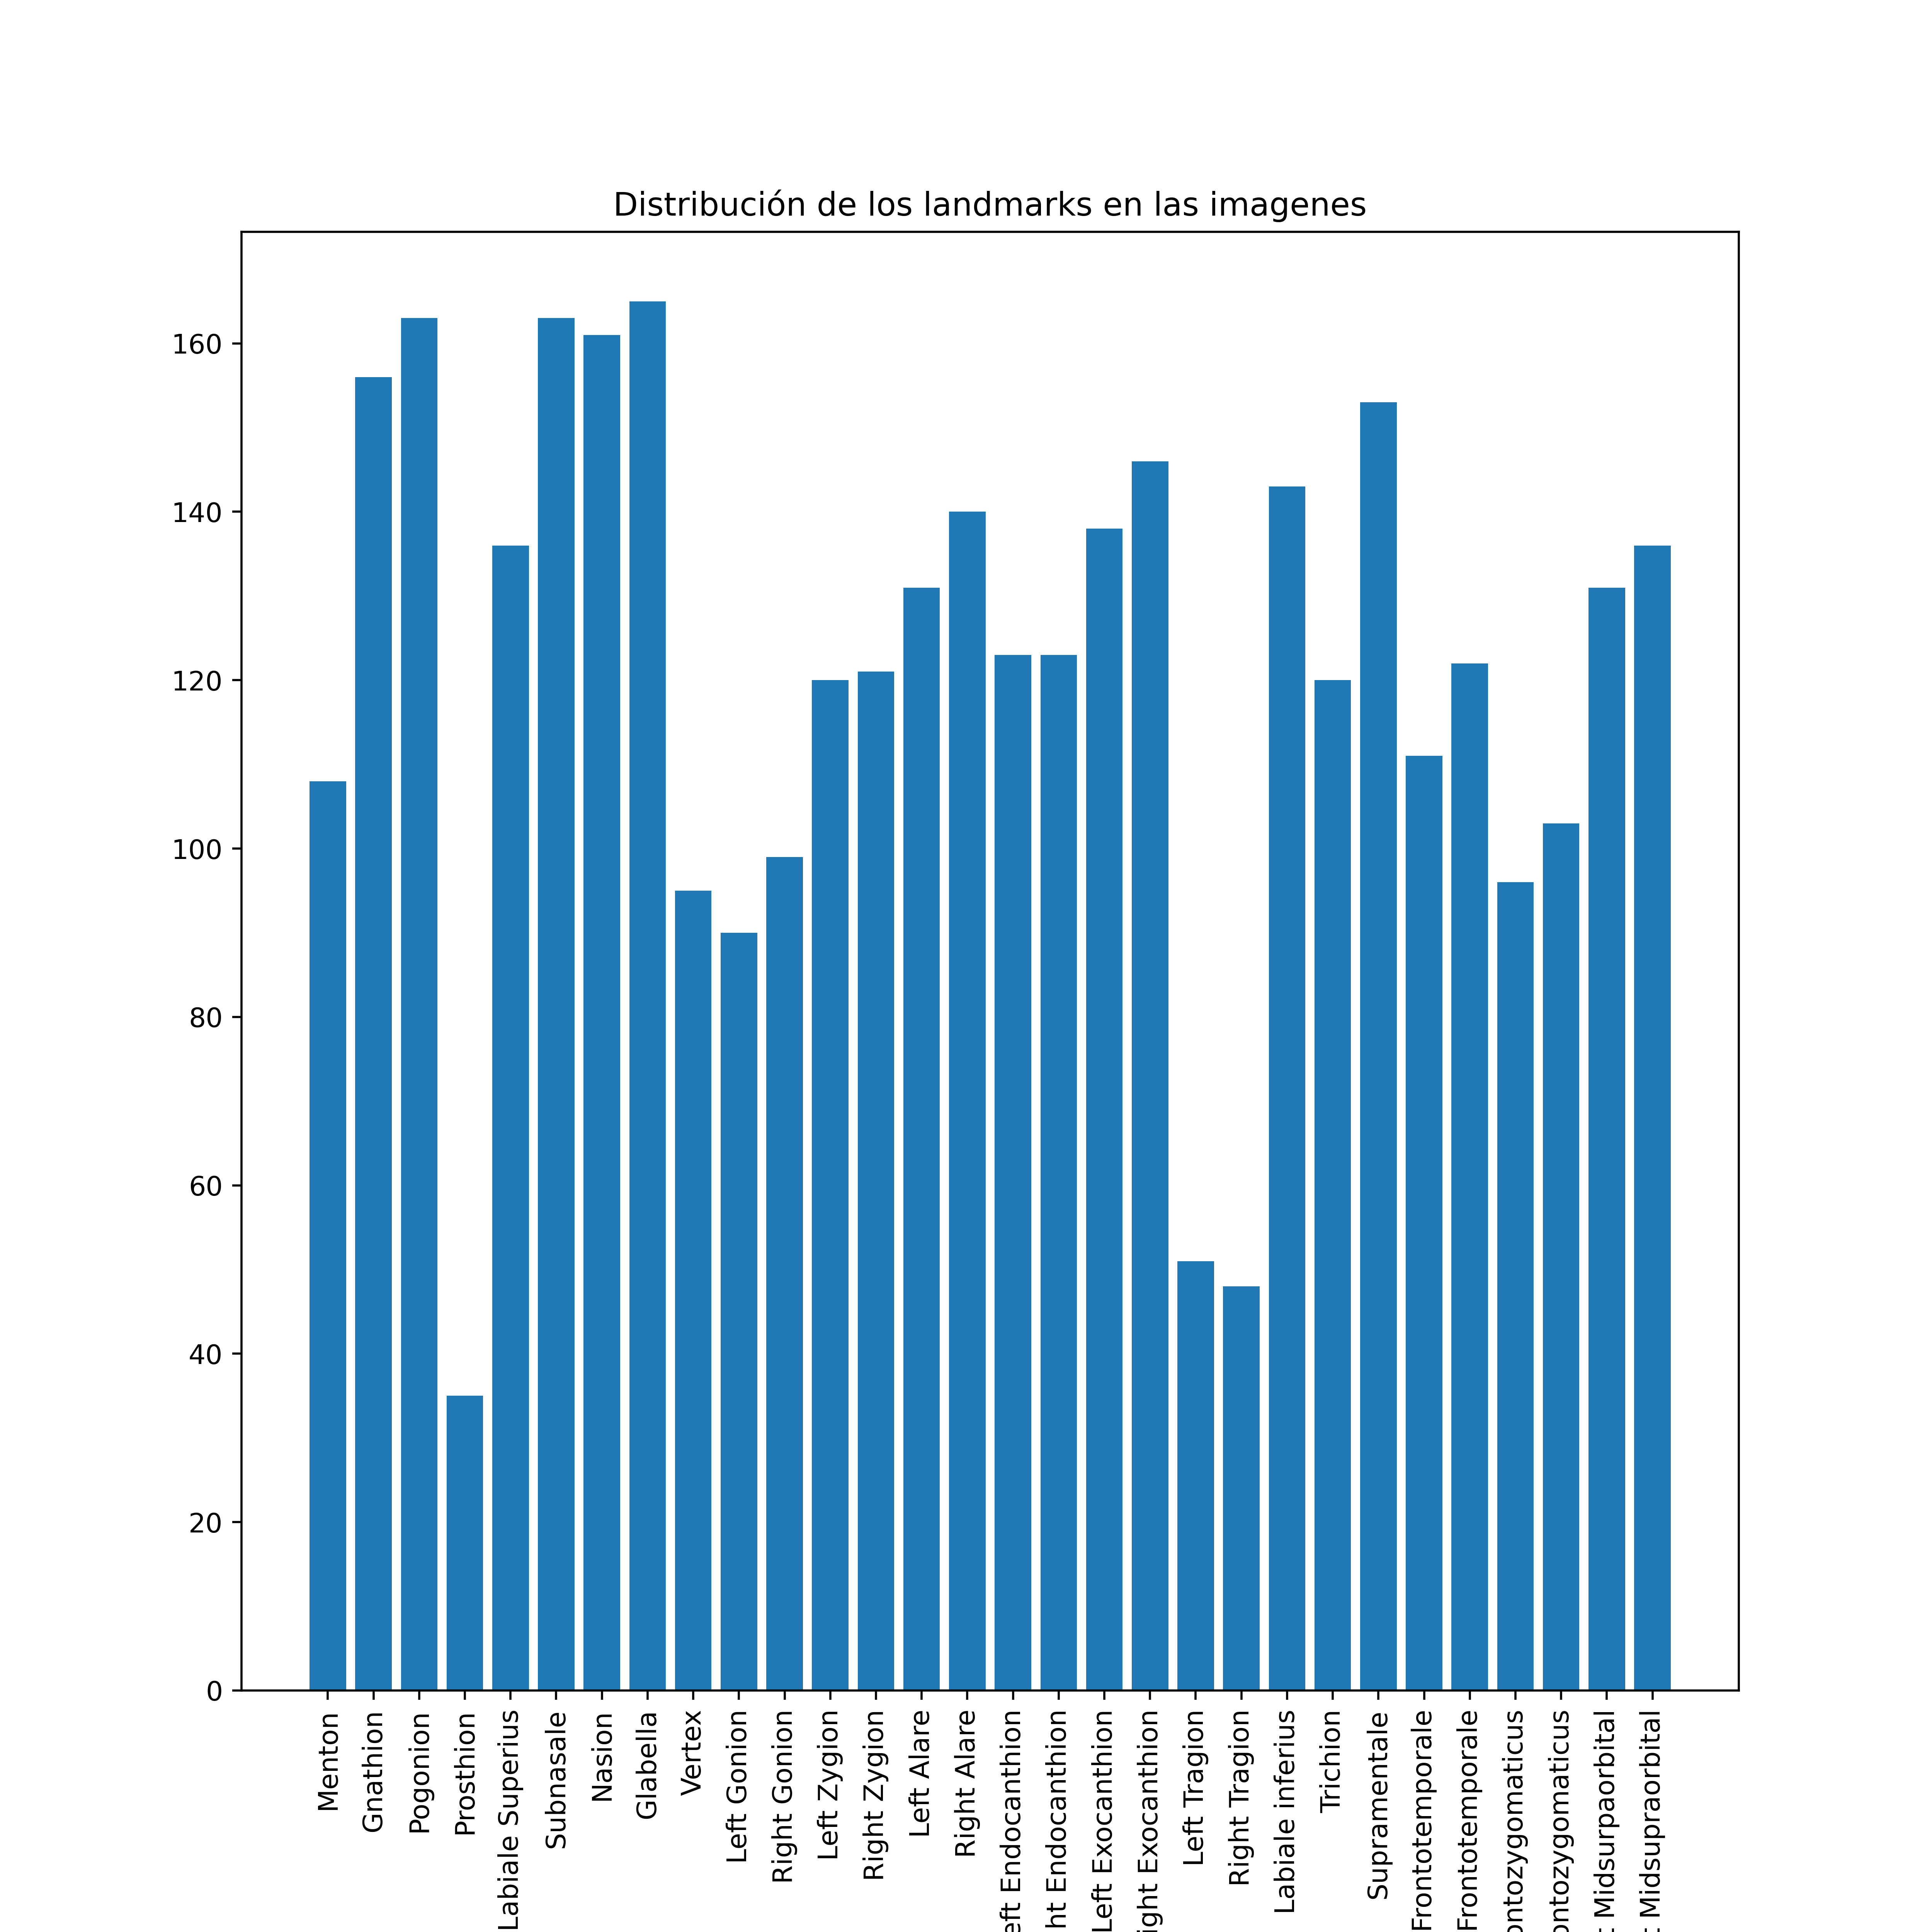
\includegraphics[width=0.7\textwidth]{img/distribucion_landmarks_imagenes.png}
                \caption{Histograma con la aparición de cada tipo de landmark en las imágenes del dataset.}
                \label{fig:Histograma}
            \end{figure}
    

\section{Requisitos mínimos del algoritmo}

\noindent El algoritmo que buscamos debería tener unos requisitos mínimos: 

\begin{itemize}
    \item Debe ser un método \textbf{robusto}, en el sentido de que debe abarcar todos los posibles casos y variaciones del problema. En nuestro caso se traduce en saber lidiar con imágenes frontales, de perfil o $3/4$ junto con otros factores como la calidad de la imagen, iluminación y oclusiones parciales. En todos los casos anteriores, el algoritmo debería tener un buen comportamiento.
    \item Capaz de operar con un \textbf{pequeño conjunto de datos}, ya que como hemos comentado anteriormente, se dispone generalmente de pocas imágenes para realizar el marcado de landmarks. Esta propiedad es deseable porque generalmente, en los problemas forenses reales, no se dispone de una amplia variedad de imágenes de la persona desaparecida, en algunos casos sólo se dispone de unas pocas imágenes y no todas van a ser frontales y con buena calidad e iluminación.

    \item Debe proporcionar siempre una solución lo más \textbf{correcta} posible.  
    
    \item Debe ser \textbf{eficaz} y \textbf{eficiente}. Buscamos acelerar el proceso del marcado de landmarks considerablemente a la par que conseguir resolver el objetivo principal.
\end{itemize}

\noindent Remarcamos que la intención no es reemplazar al experto en su labor del marcado de landmarks sino proporcionar una ayuda para acelerar el proceso.

\section{Objetivos}

\noindent Los objetivos a resolver en el trabajo son los siguientes: 

\begin{enumerate}
    \item Realizar una investigación sobre el estado del arte en la localización de landmarks cefalométricos en fotografías en el ámbito de la antropología forense.
    \item Realizar una investigación sobre los modelos de Autoencoders y redes adversarias existentes.
    \item Explorar el dataset proporcionado para identificar errores o anomalías y pre-procesar el conjunto de datos existente, con el fin de obtener un dataset apto para el entrenamiento de la red.
    \item Realizar un estudio experimental realizando diversas pruebas sobre el framework con el conjunto de datos proporcionado.
\end{enumerate}

\section{Planificación}
    \noindent La planificación del proyecto, desde un comienzo, fue pensada para llevar a cabo el desarrollo del software siguiendo un modelo en cascada, evitando la vuelta atrás entre etapas. Sin embargo, debido a que el desarrollo consistirá principalmente en una adaptación de un software ya existente, se estimó desde un principio que en esta etapa no se desarrollaría un programa de gran complejidad. Una vez adaptado el framework a nuestro objetivo, sabíamos que el software podría sufrir ligeras modificaciones en función de los resultados obtenidos durante la experimentación. Es por ello, que se optó por un modelo de ciclo de vida en cascada retroalimentado como se puede ver en \autoref{Fig::Ciclo de vida}.


    \begin{figure}[!h]
        \centering
        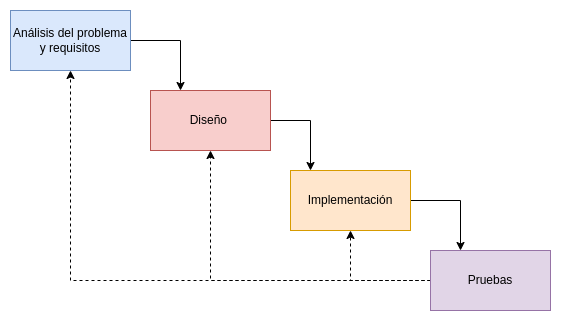
\includegraphics[width=0.8\textwidth]{img/disenio_cascada.png}
        \caption{Diseño en cascada retroalimentado empleado.}
        \label{Fig::Ciclo de vida}
    \end{figure}

    \medskip

    \noindent Las etapas que se seguirán serán las siguientes:

    \begin{enumerate}
        \item \textbf{Análisis del problema y requisitos}: En esta tapa se profundizará sobre el contexto y la importancia del problema a resolver y se llevarán a cabo reuniones con los tutores del trabajo para aclarar los requisitos y objetivos concreto del software a desarrollar. 
        \item \textbf{Diseño}: En nuestro caso, en esta etapa se realizarán dos tareas: 
        
        En primer lugar se realizará un análisis de la base de datos que emplearemos así como las transformaciones que deban sufrir los datos para poder ser empleados por el software de experimentación. 

        En segundo lugar se diseñarán los experimentos a realizar así como las técnicas que se aplicarán, las métricas y los protocolos de validación que se usarán.

        \item \textbf{Implementación}: Se implementan todas las técnicas diseñadas en la etapa anterior.
        \item \textbf{Experimentación}: Se ponen en práctica todos los experimentos diseñados de forma teórica y se obtienen resultados. En función de estos se valora una vuelta atrás en el ciclo de vida del software para realizar modificaciones en el software.
    \end{enumerate}
    
    \medskip

    \noindent Debido a la alta carga de trabajo durante el curso, desde un comienzo, el desarrollo del trabajo se planificó pensando en su defensa para la convocatoria extraordinaria de Septiembre o para la convocatoria especial de Noviembre. Por ello, la planificación original por meses se puede observar en la \autoref{Fig::Planificacion final}.


    \begin{figure}[!h]
        \centering
        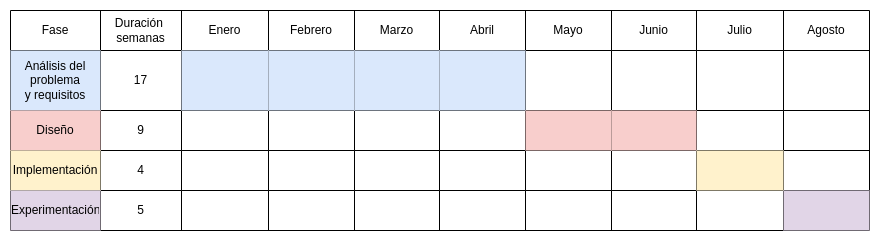
\includegraphics[width=0.9\textwidth]{img/plan_provisional.png}
        \caption{Planificación original.}
        \label{Fig::Planificacion original}
    \end{figure}

    \medskip

    \noindent Dentro de la semana computan únicamente los días de Lunes a Viernes. Resalta a la vista la gran cantidad de semanas invertidas en las primeras dos etapas con respecto a las invertidas en las dos últimas. El principal motivo para repartir el tiempo de esta manera es que durante el curso se calculó que sería imposible dedicar al trabajo más de \textbf{cuatro horas por semana}. En cambio, una vez terminado el curso se previó dedicar una media de \textbf{seis horas diarias al trabajo}. Es por ello que a pesar de la gran diferencia de semanas, si miramos las horas obtenemos:
    
    \begin{itemize}
        \item Para la primera fase se invirtieron un total de \textbf{68 horas}.
        \item Para la segunda fase un total de \textbf{36 horas}.
        \item Para la tercera y cuarta fase se invirtieron un total de \textbf{120 horas} para cada una.
        \item En total el tiempo estimado de desarrollo del proyecto fue de \textbf{344 horas}.
    \end{itemize}
        
    \noindent No obstante, esta estimación resultó ser muy ajustada para completar el trabajo, lo que ocasionó que se retrasara la entrega del mismo a Noviembre, es por ello que el plan definitivo del proyecto se puede ver en la \autoref{Fig::Planificacion final}. Aquí se puede ver cómo desde Septiembre, a causa de los resultados obtenidos en la experimentación, se vuelve atrás en el ciclo de vida del software a la parte de análisis del problema y requisitos para consultar a los tutores con los resultados obtenidos y modificar el resto de etapas sucesivas. El tiempo invertido por día en esta segunda fase fue de \textbf{4 horas} diarias. Lo que incrementa el tiempo total invertido a:

    \begin{itemize}
        \item \textbf{148 horas} para la primera fase.
        \item Para la segunda fase un total de \textbf{76 horas}.
        \item Para la tercera y cuarta fase se invirtieron un total de \textbf{160 horas} para cada una.
        \item En total el tiempo estimado de desarrollo del proyecto fue de \textbf{544 horas}.
    \end{itemize}

    \begin{figure}[!h]
        \centering
        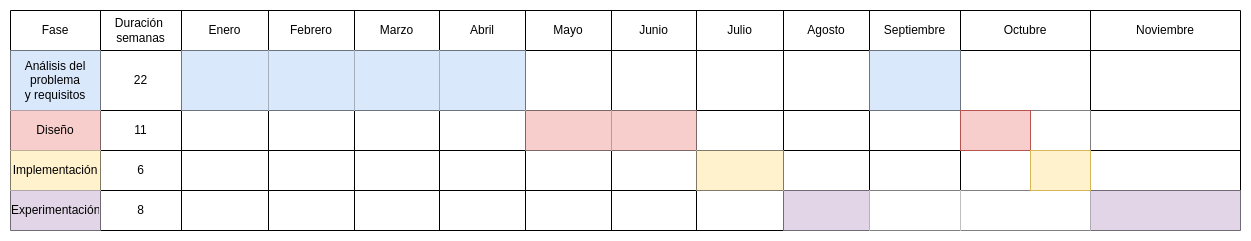
\includegraphics[width=0.95\textwidth]{img/plan_definitivo.png}
        \caption{Planificación final.}
        \label{Fig::Planificacion final}
    \end{figure}

    \medskip

    \noindent Como consecuencia, en un principio se preveía usar un total de \textbf{344} horas para finalizar el trabajo, pero finalmente hicieron falta \textbf{544} horas, de esta forma, si se supone que un Investigador en una empresa de base tecnológica es de 35€/hora, a partir de los resultados obtenidos, el trabajo tenía un presupuesto inicial de \textbf{12.040 €} que finalmente fue ampliado a \textbf{19.040 €}.

\endinput
%------------------------------------------------------------------------------------
% FIN DEL CAPÍTULO. 
%------------------------------------------------------------------------------------


